% Created 2017-04-30 Sun 21:21
% Intended LaTeX compiler: pdflatex
\documentclass[moor]{informs1}
               \usepackage{minted}
               \usepackage{tikz}
\usetikzlibrary{arrows.meta}
\usepackage{natbib}
\usepackage{listing}
\usepackage{algorithm}
\usepackage{mathtools}
\usepackage{algpseudocode}% http://ctan.org/pkg/algorithmicx
%\usepackage[noend]{algpseudocode}
\algdef{SE}[DOWHILE]{Do}{doWhile}{\algorithmicdo}[1]{\algorithmicwhile\ #1}%
\algdef{SE}[DOWHILE]{Do}{doWhile}{\algorithmicdo}[1]{\algorithmicwhile\ #1}%
\usepackage[colorlinks=true,breaklinks=true,bookmarks=true,urlcolor=blue,
citecolor=blue,linkcolor=blue,bookmarksopen=false,draft=false]{hyperref}
\def\TheoremsNumberedThrough{%
\theoremstyle{TH}%
\newtheorem{thm}{Theorem}
\newtheorem{lemma}{Lemma}
\newtheorem{prop}{Proposition}
\newtheorem{cor}{Corollary}
\newtheorem{claim}{Claim}
\newtheorem{conjecture}{Conjecture}
\newtheorem{hypothesis}{Hypothesis}
\newtheorem{assumption}{Assumption}
\newtheorem{definition}{Definition}
\newtheorem{myexample}{Example}
\newtheorem{remark}{Remark}
}
\renewenvironment{proof}{\emph{Proof.}}{END.}
\def\EMAIL#1{\href{mailto:#1}{#1}}% When hyperref is used, otherwise outcomment
\def\URL#1{\href{#1}{#1}}         % When hyperref is used, otherwise outcomment
\TheoremsNumberedThrough     % Preferred (Theorem 1, Lemma 1, Theorem 2)
\EquationsNumberedThrough    % Default: (1), (2), ...
\NatBibNumeric
\def\bibfont{\small}%
\def\bibsep{\smallskipamount}%
\def\bibhang{24pt}%
\def\BIBand{and}%
\def\newblock{\ }%
\bibpunct[, ]{[}{]}{,}{n}{}{,}%
\author{bachir el khadir}
\date{\today}
\title{}
\begin{document}

\TITLE{Time-Varying Linear and Semidefinite Programs}

\RUNAUTHOR{Ahmadi and EL Khadir}
\RUNTITLE{Time-Varying LPs and SDPs}

\ARTICLEAUTHORS{
\AUTHOR{Amirali Ahmadi}
\AFF{Princeton University, \EMAIL{aaa@princeton.edu}}
\AUTHOR{Bachir El Khadir}
\AFF{Princeton University, \EMAIL{bkhadir@princeton.edu}}
}

\ABSTRACT{
We study linear, quadratic, second order cone, and semidefinite programs whose data (e.g., the matrices $A$, $b$, $c$ in the LP case) are not constant but vary polynomially with time. We show that, under some conditions, we can approximate the optimal value of these problems arbitrarily well by searching for solutions that are polynomial functions of time themselves. Furthermore, we show that the problem of finding the optimal polynomial solution of a given degree can be cast exactly as a semidefinite program. 
}

\maketitle



\section{Introduction}
\label{sec:orgheadline4}

In this paper we investigate time varying convex programs, i.e. optimization problems for which the feasible set and the objective function depend  on time over a compact interval.

Concrete applications of this kind of problems include scheduling an electric power generation when users daily consumption is known in advance or insuring maximum cellular coverage of customers at minimum cost when geographical population density fluctuates over the course of a day.

More specifically, a time-varying linear program (abbreviated \ref{eq:orglatexenvironment1}) is defined as follow:

\begin{equation*}
\label{eq:orglatexenvironment1}
\tag{TV-LP}
\begin{array}{ll@{}ll}
\underset{x(t)}{\text{maximize}} & \int_{-1}^1 \langle c(t), x(t) \rangle dt & \\
\text{subject to}& A(t) x(t) \le b(t) & \forall t \in [-1, 1]
\end{array}
\end{equation*}

\noindent  with \(A(t) \in \mathbb R^{m \times n}, x(t), c(t) \in \mathbb R^n\) and \(b(t) \in \mathbb R^m\) for all \(t \in [-1, 1]\), and moreover, the components of \(A\), \(b\), \(c\) are polynomial functions time \(t\).

We consider the data of the problem \((A, b, c)\) to belong to the set of \emph{polynomial} functions because on the one hand, this set is dense in the set of continuous functions defined on \([0, 1]\), and on the other hand, polynomials can be parameterized in a natural way (in the monomial basis for instance) and are more suitable to algorithmic operations (see section \ref{orgtarget1}). 

The optimization variable is a function \(x: [-1, 1]\rightarrow \mathbb R^n\). When such function verifies the program constraints for all \(t \in [-1,1]\), we call it a \emph{feasible function}. 

  One numerical example of a time varying LP to consider is the following (illustrated in figure \ref{fig:orgparagraph1}):
\[
A(t) = \begin{pmatrix}
2-t&-1-t\\
1+t&2-t\\
-2+t&1+t\\
-1-t&2-t\\
2+t&2+t
\end{pmatrix}
b(t) = \begin{pmatrix}1\\1\\2\\2\\-t\end{pmatrix}
c(t) = \begin{pmatrix}t \\ t^2\end{pmatrix} \]

\begin{figure}[htb]
\centering
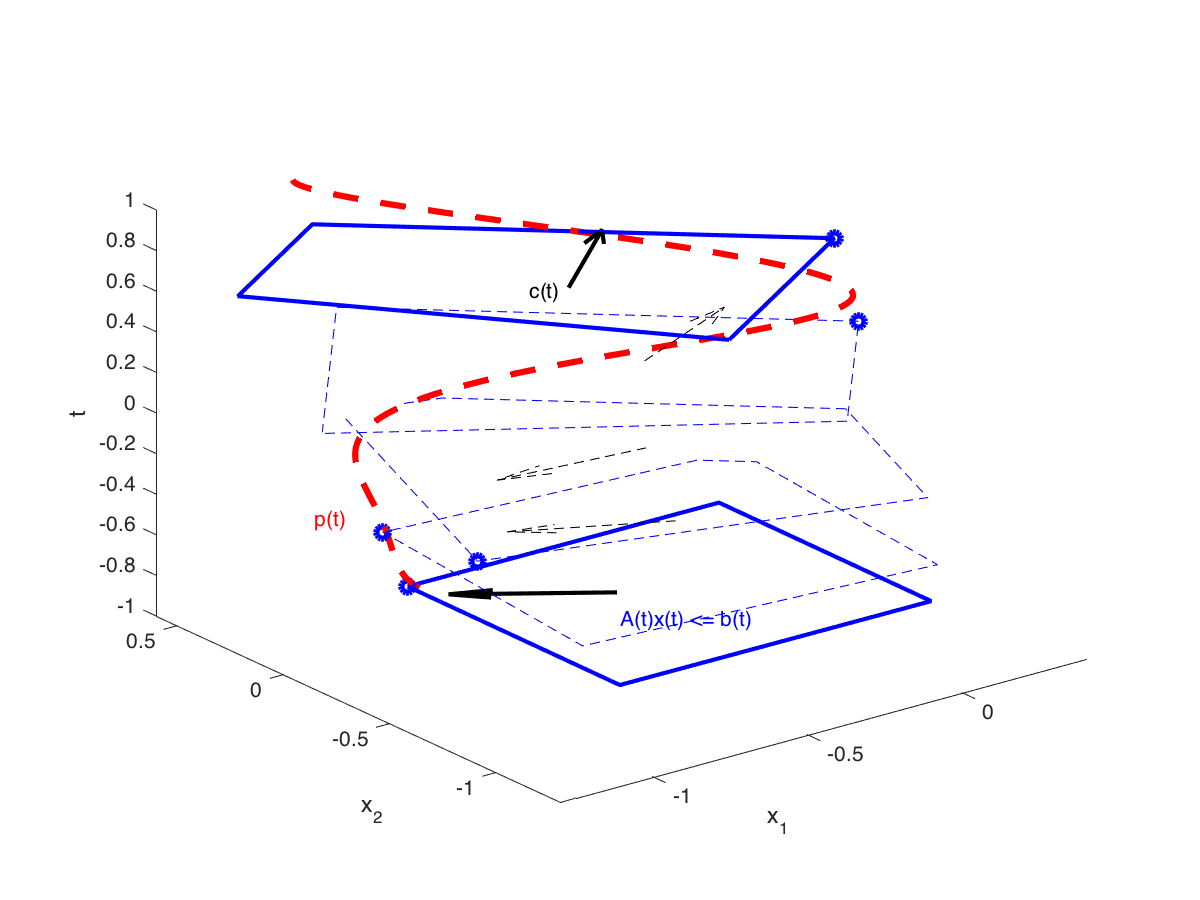
\includegraphics[width=0.5\textwidth]{scripts/example_tv_lp.png}
\caption{\label{fig:orgparagraph1}
An example of a time-varying LP}
\end{figure}


The blue circles represent the optimal solution \(x^{opt}(t)\) for each time \(t\) that maximizes \(\langle c(t), x(t)\rangle\) under the constraint \(A(t)x(t) \le b(t)\), and the dotted red line represents the optimal polynomial solution \(x^{poly}(t)\) of degree \(11\). The feasible set \(\{x \in \mathbb R^n\; |\;  A(t)x \le b(t)\}\) for any time \(t\) is delimited by blue lines. As time progresses, the number of facets of this set changes. The objective function \(c(t)\) is represented by a black arrow. 

Notice that in general the optimal solution to a time-varying LP is the function that we denote by \(x^{opt}(t)\) that maximizes the following program for almost all times \(t \in [-1, 1]\) :

\begin{equation*}
\label{eq:orglatexenvironment2}
\tag{$LP_t$}
\begin{array}{ll@{}ll}
\underset{x(t)}{\text{maximize}} & \langle c(t), x(t) \rangle & \\
\text{subject to}& A(t)x(t) \le b(t)\\
\end{array}
\end{equation*}


A time-varying semidefinite program (abbreviated \ref{eq:orglatexenvironment3}) is the following optimization problem:

\begin{equation*}
\label{eq:orglatexenvironment3}
\tag{TV-SDP}
\begin{array}{ll@{}ll}
\underset{X(t)}{\text{maximize}} & \int_{-1}^1 \langle X(t), C(t) \rangle dt & \\
\text{subject to}& X(t) \succeq 0 & \forall t \in [-1, 1]\\
& \langle A_i(t), X(t) \rangle \le b_i(t) & \forall t \in [-1, 1]
\end{array}
\end{equation*}

\noindent with \(A_i(t) , X(t), C(t) \in \mathcal S_n, b_i(t) \in \mathbb R\) for all \(t \in [-1, 1], i=1, \ldots, m\). \(A_i, b_i\) for \(i=1,\ldots,m\) and \(C\) are polynomial functions of time. 

The optimal solution to a time-varying SDP is the function that we denote by \(X^{opt}(t)\) that maximize the following program for almost all times \(t \in [-1, 1]\) :

\begin{equation*}
\label{eq:orglatexenvironment4}
\tag{$SDP_t$}
\begin{array}{ll@{}ll}
\underset{X(t)}{\text{maximize}} & \langle X(t), C(t) \rangle & \\
\text{subject to}& X(t) \succeq 0\\
& \langle A_i(t), X(t) \rangle \le b_i(t) \; i=1, \ldots, m
\end{array}
\end{equation*}


Note that time-varying LPs are a special case of time-varying SDPs, hence properties that apply to the latter apply to the former as well. We focus for the most part on time-varying LPs however because they are easier to study and provide insights into the more general problem of SDPs.

It is important to notice that in general the optimal solution to a time-varying LP \(x^{opt}(t)\) (and more generally, to a time-varying SDP \(X^{opt}(t)\)) is not polynomial, and might not even be continuous. In the example of Figure \ref{fig:orgparagraph1} for instance, the optimal solution \(x^{opt}(t)\) lives on the vertices of the feasible set and occasionally jumps from one vertex to a different one, or in other terms, there are times when the set of indices of constraints that are tight for \(x^{opt}(t)\) changes, while the optimal polynomial solution moves continuously in the feasible set and tries to be as close as possible to \(x^{opt}(t)\).


In the applications mentioned at the beginning of this introduction, one looks for a feasible function that is smooth and optimal. In this paper we discuss when solutions of this form are optimal, and in that case we use sum of squares optimization to obtain the best feasible solution whose components are polynomial of a bounded degree.

Since we are looking specifically for polynomial feasible solutions, it is necessary to settle for a weaker notion of optimality than point-wise optimality. We say that a continuous solution \(f\) for a \ref{eq:orglatexenvironment1} (resp. \ref{eq:orglatexenvironment3}) is \(\varepsilon\) -near optimal if \(\int_{-1}^1 \langle f(t), c(t)\rangle dt - \int_{-1}^1 \langle x^{opt}(t), c(t)\rangle dt \le \varepsilon\). (resp. \(\int_{-1}^1 \langle f(t), c(t)\rangle dt - \int_{-1}^1 \langle X^{opt}(t), c(t)\rangle dt \le \varepsilon\)). If for all positive \(\varepsilon\), there exist a continuous (resp. polynomial) feasible solution that is \(\varepsilon-\) near optimal for the TV-LP or TV-SDP, we say that continuous (resp. polynomial) solutions are near optimal for the TV-LP or TV-SDP.



\subsection{Notations}
\label{sec:orgheadline1}
\begin{itemize}
\item For a  integer \(n\), we denote by \([n]\) the set \(\{0, \ldots, n\}\).
\item The \(n \times 1\) vector whose component are all equal to 1 is denoted by a capital \(\bf{1}\).
\item For a matrix \(A\) of dimension \(m \times n\), \(A_i\) is the \(i^{th}\) row of \(A\) for \(i=1, \cdots, n\). If \(m \ge n\), given an index set \(B = (b_1, \ldots, b_n)\), then \(A_B\) is the \(n \times n\) sub-matrix \((A_{b_i,j})_{1 \le i, j \le n}\).
\item We denote the set of \(n \times n\) positive semidefinite matrices by \(\mathcal S_n\).
\item For \(d \in \mathbb N\), \(\mathbb R_d[y]\) is the set of polynomials in the variable \(y\) with real coefficients that have degree  at most \(d\).
\item We denote the set of polynomials of degree \(d\) in the variable \(y\) that can be written as sum of squares of some polynomials by \(SOS_d(y)\), i.e., \(SOS_d(y) = \mathbb R_d[y] \cap \sum \mathbb R[y]^2\).
\item The set \(\mathcal P_t\) is the feasible set of a \ref{eq:orglatexenvironment1} with data \((A, b, c)\) at time \(t\), i.e. \(\mathcal P_t = \{x \in \mathbb R^n | A(t) x \le b(t) \}\).
\item For a subset \(C\) of \(\mathbb R^n\), \(conv(C)\) denotes is convex hull.
\end{itemize}
\newpage

\subsection{Assumptions}
\label{sec:orgheadline2}
Throughout the paper, we make the following assumptions:
\begin{itemize}
\item For all \(t \in [-1, 1]\), \(\mathcal P_t \ne \emptyset\), i.e. there exists at least one feasible solution at time \(t\). (This condition can be checked in finite time using Algorithm \ref{orgspecialblock1})
\item For all \(t \in [-1, 1]\),  \(\mathcal P_t\) is bounded. (We show in Theorem \ref{orgspecialblock2} that the bound can be made independent of \(t\))
\end{itemize}
\newpage

\subsection{Organization and Contributions of the paper}
\label{sec:orgheadline3}
In this paper we propose an efficient method to find the best polynomial solution to a time-varying linear program or semidefinite program, as well as a characterization of when polynomial solutions are close to being optimal. The paper is organized as follow:
\begin{itemize}
\item In Section \ref{orgtarget2}, we first show that the solutions to a \ref{eq:orglatexenvironment1} are piece-wise rational functions of time (Theorem \ref{orgspecialblock3}). Then, we give equivalent conditions under which continuous solutions are feasible and optimal for a \ref{eq:orglatexenvironment1} (Theorem \ref{orgspecialblock4}), and we prove that in fact, optimality and feasibility of continuous solutions are the same (Theorem \ref{orgspecialblock5}). We also mention the sepcial case when the constraints matrix \(A(t)\) is independent of time (e.g.  \(A(t)\) is always equal to \(A(0)\)), in which case optimal polynomial solutions exist unconditionally. (Theorem \ref{orgspecialblock6}) Finally, we prove that under strict feasibility conditions, polynomial solutions exist and are optimal (Theorem \ref{orgspecialblock7}).

\item In Section \ref{orgtarget3}, we give a finite time algorithms for checking the feasibility of TV-LP (Algorithm \ref{orgspecialblock1}), checking strict feasibility of TV-LP (Section \ref{orgtarget4}), solving a TV-LP exactly (Algorithm \ref{orgspecialblock8}), and deciding feasibility of continuous solutions to a TV-LP (Section \ref{orgtarget5}).
\end{itemize}



\begin{itemize}
\item Section \ref{orgtarget1} presents an SDP formulation for finding the best polynomial solution of a \ref{eq:orglatexenvironment1}. (Theorem \ref{orgspecialblock9})
\item Section \ref{orgtarget6} discusses the case of a \ref{eq:orglatexenvironment3}s, and proves that under similar condition to time-varying a \ref{eq:orglatexenvironment1}s , polynomial solutions exist and are optimal.
\end{itemize}
\newpage


\section{Time-Varying LP}
\label{sec:orgheadline10}
\label{orgtarget2}
\subsection{Continuity of the optimal value and boundedness of the feasible set}
\label{sec:orgheadline5}

We start with two basic theorems that are going to be used in this section. The first one is due to D. H. Martin. It characterizes the continuity of the optimal value to an LP under perturbations to its data. The second theorem states that if the feasible set \(\mathcal P_t\) is bounded for all times \(t \in [-1, 1]\), then the bound can be made uniform in \(t\).

\begin{thm}
(See \cite{Martin1975}).
Consider the LP

\begin{equation*}
\label{eq:orglatexenvironment5}
\tag{LP}
\begin{array}{ll@{}ll}
\underset{x \in \mathbb R^n}{\text{maximize}} & \langle c, x \rangle\\
\text{subject to}& A x \le b
\end{array}
\end{equation*}

Let \(\Omega\) be the set of tuples \((A, b)\) for which the set \(\{x \in \mathbb R^n, Ax \le b\}\) is non empty and bounded, and \(opt(A, b, c)\) the optimal value of (\ref{eq:orglatexenvironment5}) defined for \((A, b, c) \in \Omega \times \mathbb R^n\).

The function \(opt\) is continuous with respect to the variables \(b\) and \(c\) and upper semi-continuous with respect to the variable \(A\).
\label{orgspecialblock10}

\end{thm}


\begin{thm}
Suppose that \(\mathcal P_t\) is feasible for all \(t \in [-1, 1]\). If \(\underset{x \in \mathcal P_t}{\sup} ||x|| < \infty\) for all \(t \in [-1, 1]\), then  \(\underset{x \in \underset{t \in [-1, 1]}{\cup} \mathcal P_t}{\sup} ||x|| < \infty\).
\label{orgspecialblock2}

\end{thm}

\begin{proof}
For \(t \in [-1, 1]\), consider the following maximization program $$\underset{x \in \mathcal P_t}{\text{maximize}} \sum_{i=1}^n |x_i|$$ and denote its optimal value by \(f(t)\). The function \(f(t)\) is finite for all \(t \in [-1, 1]\) and we want to prove that \(f(t)\) can be uniformly bounded on \([-1, 1]\).

Notice that this is an LP for all \(t \in [-1,1]\), and that by the assumption we made earlier, its set of solution must be bounded for all \(t \in [-1, 1]\). As a result, all conditions for Theorem \ref{orgspecialblock10} are verified, and we conclude that  the function \(f(t)\) is upper semi-continuous.

Now, if \((t_n)_{n \in \mathbb N}\) is a convergent sequence such that \(t_0 = \underset{n \rightarrow \infty}{\lim} t_n\) and \(\sup_t f(t) =  \underset{n \rightarrow \infty}{\lim} f(t_n)\), then: \(\sup_t f(t) = \lim_n f(t_n) \le f(t_0) < \infty\). We have just found a uniform bound for the function \(f(t)\) on \([-1, 1]\).
\end{proof}

Without loss of generality, we assume for the rest of this paper that we can amend the constraints \(\{-M \le x_i \le M, i=1, \ldots, n\}\) for some positive \(M \in \mathbb R\) to a \ref{eq:orglatexenvironment1}.
\newpage


\subsection{Geometry of the feasible set of a \ref{eq:orglatexenvironment1}}
\label{sec:orgheadline6}

We start be presenting the following theorem that describes the geometry of the feasible set \(\mathcal P_t\) of a \ref{eq:orglatexenvironment1}. The theorem states that, except for some finite number of times, the feasible set is a convex combination of points that move as rational functions in time. More formally:

\begin{thm}
Consider a \ref{eq:orglatexenvironment1} with data \((A, b, c)\) and feasible set \(\mathcal P_t\) at time \(t \in [-1, 1]\).

There exist \(N\) break points \(-1 = t_1 < \cdots < t_N = 1\) and \(N-1\) finite sets of rational functions \(\mathcal V_1, \ldots, \mathcal V_{N-1} \subset \mathbb R^n(X)\) such that, for every \(i \in \{ 1, \ldots, N-1\}\), for \(t \in (t_i, t_{i+1})\), the feasible set \(\mathcal P_t\) is the convex hull of the set of vertices \(\{v(t), \; v \in \mathcal V_i\}\).

Furthermore, for every \(i\) in \(\{ 1, \ldots, N-1\}\), every element \(v\) of the set \(\mathcal V_i\) can be associate with a subset \(B_v \subseteq [m]\) such that \(v(t) = A_{B_v}(t)^{-1}b(t)\) for  \(t \in (t_i, t_{i+1})\).
\label{orgspecialblock3}

\end{thm}

\begin{proof}
At any given time \(t \in [-1, 1]\), \(\mathcal P_t\) is a bounded polyhedron, so it is equal to the convex hull of its vertices. All vertices can be written as: \(A_B(t)^{-1}b(t)\) for some \(B \in  {[m] \choose n}\), i.e. for all \(t \in [-1, 1]\), there exists a finite set \(\mathcal B(t)\) such that \(\mathcal P_t = conv\{A_B(t)^{-1}b(t), B \in \mathcal B(t)\}\).

It remains to show that \(\mathcal B(t)\) changes at most finitely many times, which would prove the claim of the theorem. Indeed, that set changes at time \(t_0\) only if one of these two things happen for some \(B \in  {[m] \choose n}\):
\begin{itemize}
\item A nonzero polynomial of the form \(t \rightarrow \det(A_B(t))\) equals \(0\) at \(t_0\).
\item One of the components of \(t \rightarrow b(t) - A_B(t)^{-1}b(t)\) changes sign at \(t_0\). (With the convention \(A_B(t)^{-1} = I_n\) when \(A_B(t)\) is not invertible)
\end{itemize}
Both things happen only finitely many times.
\label{orgspecialblock11}

\end{proof}

Even though the previous theorem gives a description of the feasible set and ignores the objective function, it is not very hard to see that the optimal solution can also be chosen to be a piece-wise rational function in \(t\). Indeed, there always exist an optimal solution of a linear program on a vertex, and if \(c(t)\) is ``nice'' enough, e.g. a polynomial, optimality of any given vertex changes only finitely many time inside \([-1, 1]\).

\begin{thm}
Consider a \ref{eq:orglatexenvironment1} with data \((A, b, c)\). There exist breakpoints \(-1 = t_1 < \cdots < t_N = 1\) and \(N-1\) sets of rational functions \(\mathcal V_1, \ldots, \mathcal V_{N-1}\) such that the following holds:

For all \(i = 1, \ldots, N\), there exist \(v \in \mathcal V_i\) such that for every \(t \in (t_i, t_{i+1})\), the optimal value at time \(t\) of the \ref{eq:orglatexenvironment1} is achieved at the point \(v(t)\).

In other terms, we can take the optimal solution  \(x^{opt}(t)\) of the \ref{eq:orglatexenvironment1} to be equal to \(A_{B_i}(t)^{-1}b(t)\) for \(t \in (t_i, t_{i+1})\), where \(B_i \subseteq [m]\) is a set of \(n\) indices.
\label{orgspecialblock12}

\end{thm}

The theorem defines \(x^{opt}(t)\) everywhere except on the times \(t_i\). We could extend it at \(t_i\) by taking the left or right limit for example (that exist, since \(x^{opt}\) is a bounded piece-wise rational function), call this function \(\bar x^{opt}(t)\). Even though feasibility of \(\bar x^{opt}(t)\) will be preserved on the interval \([-1, 1]\), point-wise optimality (i.e. optimality with respect to the objective \(\langle c(t), \bar x^{opt}(t) \rangle\) for all \(t \in [1-, 1]\) ) may not be as the following example shows.

\begin{myexample}
Consider a \ref{eq:orglatexenvironment1} with objective \(c(t) = 1\) and two constraints \(-t \le tx(t) \le t, -2 \le x(t) \le 2\).
The unique point-wise optimal solution \(x^{opt}\)  to this \ref{eq:orglatexenvironment1} is

\[x^{opt}(t) = \left\{\begin{array}{cc}1&t \ne 0\\2&t = 0\end{array}\right..\]

The value \(x^{opt}(t)\) takes at \(0\) is neither the left nor the right limit at that point.
\end{myexample}

This is not a problem in our framework however, since we are mainly concerned by the average optimal value in time: \(\int_{-1}^1 \langle c(t), x^{opt}(t) \rangle dt\), and changing \(x^{opt}(t)\) at a set of measure 0 will not change that value. In the case where we are interested in maximizing the worst case: \(\min_{t \in [-1, 1]} \langle c(t), x(t) \rangle\), we can notice that $$\langle c(t_i), x^{opt}(t_i)\rangle \ge \min_{t \in [-1, 1] \setminus \{t_1, \ldots, t_N\}} \langle c(t), x^{opt}(t) \rangle, \; \forall i \in \{1, \ldots, N\}.$$
Therefore we don't lose by extending \(x^{opt}\) in this way neither.
\newpage

\subsection{Existence of continuous feasible solutions}
\label{sec:orgheadline7}
We are interested in the existence of polynomial solutions. One natural question to ask is whether such a solution always exist. The answer to that question is negative, and we prove that in fact even continuous solutions might not exist.

\begin{myexample}
Consider the \ref{eq:orglatexenvironment1} with two constraints: \(tx \ge 0\) and \(t(x-1) \ge 0\) for \(t \in [-1, 1]\). The \ref{eq:orglatexenvironment1} does not have a continuous feasible solution. We can see that by observing that the feasible set of this \ref{eq:orglatexenvironment1}  is \([1, \infty)\) when \(t > 0\) and \((-\infty, 0]\) when \(t < 0\).
\end{myexample}

The reason no continuous solution exist is that the \(\mathcal P_t\) are ``disconnected'' at 0, for a solution to exist, it has to ``jump'' at time 0. The following theorem formalizes this notion of continuity of sets and existence of continuous solutions.

\begin{thm}
Fix a \ref{eq:orglatexenvironment1} with data \((A, b, c)\). Let \(\mathcal P_t\) be its feasible set at time \(t\), and let  \(\mathcal V_1, \ldots, \mathcal V_{N-1}\) be the sets of rational functions defined by Theorem \ref{orgspecialblock3}.

The following statements are equivalent:
\begin{enumerate}
\item the \ref{eq:orglatexenvironment1} admits a continuous feasible solution.
\item \(\underset{\alpha \rightarrow 0}{\lim} dist(\mathcal P_{t_i-\alpha}, \mathcal P_{t_i+\alpha}) = 0\) for \(i = 1, \ldots, N-1\).
\item \(conv \{ v(t_{i}), v \in \mathcal V_i\} \cap conv \{ v(t_{i}), v \in \mathcal V_{i+1}\} \ne \emptyset\) for \(i = 1, \ldots, N-1\).
\end{enumerate}
\label{orgspecialblock4}

\end{thm}

\begin{proof}
We prove the theorem by proving the three implications   1 \(\implies\) 2 \(\implies\) 3 \(\implies\) 1.

(1 \(\implies\) 2)
Let \(x(t)\) be a continuous solution to our \ref{eq:orglatexenvironment1}, then \(\underset{\alpha \rightarrow 0}{\lim} dist(P_{t_i-\alpha}, P_{t_i+\alpha}) \le \underset{\alpha \rightarrow 0}{\lim} dist(x(t_i-\alpha), x(t_i+\alpha))= 0\)

(3 \(\implies\) 2)
Fix \(i\) in \(\{1, \ldots N-1\}\).
We are first going to construct a continuous solution \(x_i(t)\) that is defined for \(t \in (t_{i-1}, t_{i+1})\).
By assumption, the intersection of \(conv \{ v(t_{i}), v \in \mathcal V_i\}\) and \(conv \{ v(t_{i}), v \in \mathcal V_{i+1}\}\) is non-empty, therefore there exist two sets of non negative coefficients \((\lambda_v)_{v \in \mathcal V_i}\) and \((\lambda_v)_{v \in \mathcal V_{i+1}}\) that sum up to one such that
$$\sum_{v \in \mathcal V_i}  \lambda_{v} v(t_i) = \sum_{v \in \mathcal V_{i+1}}  \mu_{v} v(t_i).$$

For \(t \in (t_{i-1}, t_{i+1})\), define \(x_i(t)\) to be the following function

\[x_i(t) \coloneqq \left\{\begin{array}{cc}
   \sum_{v \in \mathcal V_i} \lambda_v v(t) & t \le t_i\\
   \sum_{v \in \mathcal V_{i+1}} \mu_v v(t) & t > t_i
   \end{array}\right. .
   \]

It is clear that \(x_i\) is feasible for our \ref{eq:orglatexenvironment1} and continuous on its domain, i.e. \(\lim_{t < t_i} x_i(t) = \lim_{t > t_i} x_i(t)\).


We get a continuous feasible solution on \([-1, 1]\) simply by ``connecting'' two solution \(x_i\) and \(x_{i+1}\) by interpolating from one to the other linearly.

(2 \(\implies\) 3)
Let \(i\) in \(\{1, \ldots N-1\}\), and let \(\alpha_p \coloneqq \frac1p\) for \(p \in \mathbb N\).

By assumption, \(\underset{p \rightarrow \infty}{\lim} dist(\mathcal P_{t_i-\alpha_p}, \mathcal P_{t_i+\alpha_p}) = 0\). For a positive integer \(p\), define two sequences  \((x_p)_p \in (P_{t_i-\alpha_p})^{\mathbb N}\) and \((y_p)_p \in (P_{t_i+\alpha_p})^{\mathbb N}\) such that \(\underset{p \rightarrow \infty}{\lim}{||x_p - y_p||} = 0\). Furthermore, without loss of generality, assume that \(x_p\) and \(y_p\) have a limit \(\alpha=0\). Call \(l\) their common limit.

By definition of \(\mathcal V_i\), there exist convex coefficients \(\{\lambda_v^p, v \in \mathcal V\}\) such that $$x_p = \sum_{v \in \mathcal V}\lambda^p_v v(t_i-\alpha).$$
Again, without loss of generality, assume for all \(v \in \mathcal V_i\) that the sequence \((\lambda_v^p)_p\) converges to a scalar \(\lambda_v\). As a result of taking limits of both side of the previous equality, we get that
$$l = \sum_{v \in V} \lambda_v v(t_i).$$

In the same way, we prove that there exist convex coefficients \(\{\mu_v, v \in \mathcal V_{i+1}\}\) such that \(l = \sum_{v \in \mathcal V_{i+1}} \mu_v v(t_i)\).

We have just proved that \(conv \{ v(t_{i}), v \in \mathcal V_i\} \cap conv \{ v(t_{i}), v \in \mathcal V_{i+1}\}\).
\end{proof}

A particular special case that is worth mentioning is when the matrix of constraints \(A(t)\) of a \ref{eq:orglatexenvironment1} doesn't depend on the time variable \(t\). In that case, continuous feasible solutions always exist.

\begin{thm}
For a \ref{eq:orglatexenvironment1}, if the constraints matrix \(A(t)\) doesn't depend on \(t\) then the  \ref{eq:orglatexenvironment1} admits at least one continuous feasible solution.
\label{orgspecialblock6}

\end{thm}

\begin{proof}
Assume for the sake of contradiction that no continuous feasible solution exist for a \ref{eq:orglatexenvironment1} with a constant constraints matrix \(A\), then, by Theorem \ref{orgspecialblock4}, there  exists \(i \in [m]\) such that the two polytopes \(conv \{ v(t_{i}), v \in \mathcal V_i\}\) and \(conv \{ v(t_{i}), v \in \mathcal V_{i+1}\}\) have empty intersection. As a result, there is a separating hyperplane with normal \(u \in \mathbb R^n\) and a positive scalar \(\delta\) such that \(\langle v(t_i) , u \rangle > \delta\) for \(v \in \mathcal V_i\) and \(\langle v(t_i) , u \rangle < -\delta\) for \(v \in \mathcal V_{i+1}\).


That contradicts the fact that the following LP has an optimal value that is continuous with respect to the parameter \(\alpha\) in the neighborhood of 0 (because of Theorem \ref{orgspecialblock10}):
$$\underset{x \in P_{t+\alpha}}{\text{minimize}} \langle x, u \rangle.$$
\end{proof}

Now that we have established the conditions for the existence of feasible continuous solution to a \ref{eq:orglatexenvironment1}, we will investigate additional conditions to also guarantee near optimality of continuous solutions.

It turns out that  whenever there exists one feasible continuous solution, there also exists near optimal continuous solution.

\begin{thm}
Suppose a \ref{eq:orglatexenvironment1} with data \((A, b, c)\) admits a feasible continuous solution \(f_0\), i.e. there exists a continuous function \(f_0: [-1, 1] \rightarrow \mathbb R^n\) such that \(A(t)f_0(t) \le b(t)\), \(\forall t \in [-1, 1]\).

Then, for every \(\varepsilon > 0\), there exists a continuous function \(f: [-1, 1] \rightarrow \mathbb R^n\) that is feasible and \(\int_0^1 \langle c(t), x(t)\rangle - \int_0^1 \langle c(t), f(t)\rangle \le \varepsilon\).
\label{orgspecialblock5}

\end{thm}

\begin{proof}
Fix a \ref{eq:orglatexenvironment1} that has a feasible continuous solution \(f_0\) on \([-1, 1]\).
Following the result of Theorem \ref{orgspecialblock3}, there exists  a partition  of \([-1, 1]\) with break points \(t_1, \ldots, t_N\) and an optimal solution \(x^{opt}(t)\) that is continuous on every interval \((t_i, t_{i+1})\).

We want to construct a function that is as close as possible to \(x^{opt}\) (for the norm of \(L_2([-1, 1])\) ) while staying continuous, which would prove the claim of the theorem.

For this purpose, define the interval \(I_i^{\alpha} \coloneqq (t_i+\alpha, t_i -\alpha)\) for some positive scalar \(\alpha\).

Let \(f^{\alpha}\) be the function that is equal to \(x^{opt}(t)\) on every \(I_i^{\alpha}\), equal to \(f_0\) on all the \(t_i\) and interpolates linearly between \(x(t)\) and \(f_0(t)\) on \([t_i-\alpha, t_i+\alpha]\).

In a sense, \(f^{\alpha}\) lives on the optimal vertex but ``travels'' to the continuous solution \(f_0\) to get through the possibly problematic time \(t_i\).

As \(\alpha \rightarrow 0\), \(f^{\alpha}(t) \rightarrow x^{opt}(t)\) almost surely on \([-1, 1]\). Given that the inequality \(|f^{\alpha}(t)| \le |x(t)| + |f_0(t)|\) holds for all \(t \in [-1, 1]\), the Dominated Convergence theorem gives \(f^{\alpha}(t) \rightarrow_{L_2} x(t)\), and we conclude by Cauchy-Schwarz that for any \(\varepsilon > 0\), if we take \(\alpha\) small enough, \(f^{\alpha}\) is \(\varepsilon\) -near optimal .
\end{proof}
\newpage


\subsection{A simple condition that guarantees existence and optimality of continuous solutions}
\label{sec:orgheadline8}

In this section we present a simple condition under which continuous feasible solutions to a \ref{eq:orglatexenvironment1} exists. The condition can be stated as a feasibility problem of a new \ref{eq:orglatexenvironment1}, described in the following definition, with slightly tighter constraints.

\begin{definition}
A \ref{eq:orglatexenvironment1} is \emph{strictly feasible} if there exists a (not necessarily continuous) function \(x^s: [-1, 1] \rightarrow \mathbb R^n\)   and a scalar \(\varepsilon > 0\) such that

$$A(t)x^s(t) \le b(t) - \varepsilon 1, \; \forall t \in [-1, 1].$$

\noindent In this case we say that \(x^s(t)\) is strictly feasible for our \ref{eq:orglatexenvironment1}.
\label{orgspecialblock13}

\end{definition}

The condition of existence of continuous solution to a \ref{eq:orglatexenvironment1} can now be formulated as follow:

\begin{thm}
If a \ref{eq:orglatexenvironment1}  is strict feasibility, then it has a continuous near optimal solution.
\label{orgspecialblock14}

\end{thm}

\begin{proof}
Assume strict feasibility of a \ref{eq:orglatexenvironment1}.

By Theorem \ref{orgspecialblock5}, it is enough to prove the existence of a continuous feasible solution \(x^c(t)\) to our \ref{eq:orglatexenvironment1}.

Recall from Theorem \ref{orgspecialblock3} that there exists an integer \(N > 0\), and breakpoints \(-1 = t_1 < \cdots < t_N = 1\) such that, for all \(i = 1, \ldots, N\), there exist a finite set of rational functions \(\mathcal V_i\) (the vertices) such that \(\mathcal P_t = conv\{ u(t), u \in \mathcal V_i \}\) for all \(t \in (t_i, t_{i-1})\).

We provide a construction of \(x^c(t)\) in two steps depending on whether we are near the problematic points \(t_i\), \(i = 2, \ldots, N-1\) or far away from them, then we connect these patches by interpolating between them. 

\paragraph{Near the problematic points $t_i$:}

The polytope \(\{x \in \mathbb R^n |  A(t_i)x \le b(t_i) - \varepsilon 1\}\) is not empty by strict feasibility. Let \(w\) be one of its extreme points. Then there exists a basis \(B\) such that \(w = A_B(t_i)^{-1}(b(t_i) - \varepsilon 1)\).

Now define \(w_i^{near}(t) \coloneqq A_B(t)^{-1}(b(t) - \varepsilon 1)\), then there exists a neighborhood of \(t_i\), \([t_i-\alpha, t_i+\alpha]\), such that (i) \(w_i^{near}(t)\) is a well defined continuous function and (ii) \(w_i^{near}(t)\) is strictly feasible.

Indeed, (i) is true because  \(\det(A_B(t_i)) \ne 0\) implies that \(\det(A_B(t)) \ne 0\) in the vicinity of \(t_i\). To see why (ii) is true, we observe that since \(A(t_i)w_i^{near}(t_i) \le b(t_i) - \varepsilon 1\), the inequality \(A(t)w_i^{near}(t) \le b(t) - \frac{\varepsilon}2 1\) remains true when \(t\) is arbitrarily close to \(t_i\).

Furthermore, since the number of breakpoints \(t_i\) s is finite, we can make the same choice of \(\alpha\) for all \(i = 1, \cdots, N\).

\paragraph{Far away from the $t_i$:}

For  \(t \in (t_i, t_{i+1})\), let \(w_i^{far}(t) \coloneqq \frac{\sum_{u \in \mathcal V_i} u(t)}{|\mathcal V_i|} \in \mathcal P_t\).

\noindent Let's prove that  \(w_i^{far}\) is strictly feasible on \(J_i \coloneqq [t_i+\beta, t_{i+1}-\beta]\), with \(\beta\) equal to (say) \(\min_{i=2,\ldots, N-1} \frac{t_{i+1}-t_i}{3}\).

\noindent Let
$$\delta_i^{} \coloneqq \min_{t \in J_i, j=1,\ldots, m} (b(t) - A(t)w_i^{far}(t))_j.$$
Observe that \(\delta_i > 0\). Otherwise, by continuity, there exist \(\hat j\) and \(\hat t \in J_i\) such that \((b(\hat t) - A(\hat t)w^{right}(\hat t))_{\hat j} = 0\), which means that 
\(0 = b_{\hat j}(\hat t)- A_{\hat j}^T(\hat t)w^{right}(\hat t) = \frac1{|\mathcal V_i|} \sum_{u \in \mathcal V_i} \underbrace{(b_{\hat j}(\hat t) - A_{\hat j}(\hat t)^Tu(\hat t))}_{\ge 0}\), i.e. all \(\mathcal P_t\) 's vertices belong to same affine hyper plane \(\{x \in \mathbb R^n |\; A_{\hat j}(\hat t)^T x = b_{\hat j}(\hat t) \}\), which contradicts the existence of a strictly feasible point \(x^s(t)\).

\paragraph{Connecting the patches:}

We get a continuous feasible solution on \([-1, 1]\) simply by ``connecting'' the solutions \(w_i^{far}, w_i^{near}\) by interpolating from one to the other. 

To ease notation, we can assume without loss of generality that \(\alpha = 2 \beta\). We also define the function \(I_a^b(t)\) to be the linear function equal to \(0\) at \(t = a\), and to \(1\) at \(t = b\).


Define \(x^c(t)\) to be the continuous function defined as follow:



\[x^c(t) = \left\{\begin{array}{cc}
   w_i^{far}(t) & \max(-1, t_{i-1}+2\beta) \le t \le t_{i} - 2\beta\\
   I_{t_{i} - 2\beta}^{t_{i} - \beta}(t) (w_i^{near}(t) - w_i^{far}(t)) + w_i^{far}(t) & t_{i}-2\beta < t \le t_{i} - \beta\\
   w_i^{near}(t) & t_{i}-\beta < t \le \min(1, t_{i} + \beta)\\
   \end{array}\right.
   \]


It is easy to see that \(x^c(t)\) is continuous. Furthermore, at all times \(t \in [-1, 1]\), \(x^c(t)\) is a convex combination of solutions that are strictly feasible, so that \(x^c(t)\) is also \(\varepsilon'-\) strictly feasible with  \(\varepsilon' \coloneqq \min(\varepsilon/2, \min_{i=1,\cdots,N} \delta_i)\).
\end{proof}
\newpage



\subsection{From continuous solutions to polynomial solutions}
\label{sec:orgheadline9}
\label{orgtarget7}
Our goal in this section is to understand when a \ref{eq:orglatexenvironment1} has a near optimal polynomial solution. Existence of near optimal continuous solutions is a necessary condition but unfortunately not sufficient as the following simple example shows. 

\begin{myexample}
Consider the following \ref{eq:orglatexenvironment1} with two constraints: \((1+t^2) x(t) \le 1, -(1+t^2) x(t) \le -1, \forall t \in [-1, 1]\). Clearly the only feasible solution is the continuous function \(x(t) = \frac1{1+t^2}\). However, this \ref{eq:orglatexenvironment1} does not admit a feasible (let alone optimal) polynomial solution.
\end{myexample}

To avoid such examples we need to make sure that the continuous solution can be approximated with a polynomial function that stays inside the feasible set. This motivates the following definition

\begin{definition}
A \ref{eq:orglatexenvironment1} with feasible set \(\mathcal P_t\) at time \(t \in [-1, 1]\) is \emph{continuously full-dimensional} if there exists a scalar \(\delta > 0\) and a \emph{continuous} function \(x^c: [-1, 1] \rightarrow \mathbb R^n\) such that \(B(x^c(t), \delta) \subset \mathcal P_t, \; \forall t \in [-1, 1]\).
\label{orgspecialblock15}

\end{definition}


The condition that \(\delta\) does not depend on \(t\), as well as continuity of \(x^c(t)\), are important. The following example demonstrates that.

\begin{myexample}
Consider a \ref{eq:orglatexenvironment1} with two constraints \(-2 \le x(t) \le 2, tx(t) \ge 0\) for all \(t \in [-1, 1]\). The feasible set here at time \(t\), \(\mathcal P_t\), is \(\mathbb R^+\) for \(t > 0\), \(\mathbb R^-\) for \(t < 0\), and the whole real line \(\mathbb R\) when \(t=0\).

This program is not continuously full-dimensional. Indeed, every continuous solution to this program has to be equal to 0 at \(t=0\). Now for every \(\delta > 0\), for \(t>0\) arbitrary close to \(0\), \(x(t) < \frac{\delta}2\), and therefore the ball \(B(x(t), \delta)\) cannot stay inside the feasible set at time of this \ref{eq:orglatexenvironment1}.

Notice however that the feasible continuous solution \(x(t) = t\) verifies \(B(x(t), \delta_t) \subset \mathcal P_t\), with \(\delta_t = \frac t2\) for \(t \ne 0\) and \(\delta_0 = 1\). Moreover, the feasible (non-continuous) solution
\[x(t) = \left\{\begin{array}{cc}1 & t > 0\\0&t=0\\-1&t<0\end{array}\right.\]
verifies \(B(x(t), 1) \subset \mathcal P_t\) with  for \(t \in [-1, 1]\).
\end{myexample}

We show next that full-dimensionality is exactly what is needed for the existence of the optimality of polynomial solutions.

\begin{thm}
Suppose a \ref{eq:orglatexenvironment1} is continuously full-dimensional, and denotes its optimal value by \(opt\)

Then, for every \(\varepsilon > 0\), there exists a polynomial function \(p: [-1, 1] \rightarrow \mathbb R^n\) such that  \(p(t)\) is feasible to our \ref{eq:orglatexenvironment1}, and \(\int_{-1}^1 \langle c(t), p(t)\rangle dt - opt \le \varepsilon\).
\label{orgspecialblock16}

\end{thm}


\begin{proof}
We start with a continuous solution \(g\) that is \(\varepsilon/3\) -near optimal to our \ref{eq:orglatexenvironment1},  whose existence is guaranteed by Theorem \ref{orgspecialblock5}. Ideally we would like to approximate \(g\) uniformly by a polynomial \(p\), but \(p\) might not be feasible. To correct this problem, we replace \(g\) by a convex combination of \(g\) and \(x^s\), the strictly feasible solution. Define \(f \coloneqq \lambda g + (1-\lambda) x^s\), and notice that for \(\lambda < 1\), \(g\) is strictly feasible, but when \(\lambda\) is close to 1, \(f\) is also \(\varepsilon/2\) -near optimal. 


By Weierstrass approximation theorem, let \(p(t)\) be a polynomial that approximates \(g(t)\) uniformly, i.e., \(\forall t \in [-1, 1] \; ||p(t) - f(t)||_2^2  \le \delta^2\), where \(\delta\) is a constant we are going to fix latex.

For \(\delta\) smaller than \(\varepsilon/2\), \(p(t)\) is inside \(\mathcal P_t\) for all \(t \in [-1, 1]\).

Let's now examine the objective value of \(f\):
$$\int_{-1}^1 \langle c(t), f(t)\rangle \le  \int_{-1}^1 \langle c(t), p(t)\rangle + \int_{-1}^1 ||f(t) - p(t)||_2 ||c(t)||_2 dt \le \varepsilon/2 + \delta \int_{-1}^1 ||c(t)||_2 dt$$

Again, taking \(\delta < \frac{\varepsilon/2}{1+\int_{-1}^1 ||c(t)||_2 dt}\) gives the result.
\end{proof}



A natural question here is how Definition \ref{orgspecialblock15} of continuous full-dimensionality compares to Definition \ref{orgspecialblock13} of strict feasibility, and if strict feasibility also guarantees the optimality of polynomial solutions as it does for continuous solutions. The rest of this section is devoted to this two questions.

While Definition \ref{orgspecialblock13} provides slackness in the space of the constraints, \ref{orgspecialblock15} requires the existence of a continuous solution with a ball with fixed radius around it that stays feasible for all times.

We can easily see that for any \ref{eq:orglatexenvironment1}, full-dimensionality of a continuous solution implies strict feasibility when for all \(t \in [-1, 1]\), none of the rows of the constraints inequality \(A(t)\) are identically zero.

\begin{thm}
If a \ref{eq:orglatexenvironment1} is continuously full-dimensional and has a constraint matrix with non-identically zero rows for all \(t \in [-1, 1]\), then the \ref{eq:orglatexenvironment1} is strictly feasible.
\end{thm}

\begin{proof}
Fix a continuously full-dimensional \ref{eq:orglatexenvironment1} with data \((A, b, c)\) and feasible set \(\mathcal P_t\) at time \(t \in [-1, 1]\). Let \(\delta\) be positive scalar and  \(x^c: [-1, 1] \rightarrow R^n\) a continuous feasible solutions for this \ref{eq:orglatexenvironment1} such that \(B(x^c(t), \delta) \subset \mathcal P_t\) for all \(t \in [-1, 1]\).


Let's define
$$\varepsilon \coloneqq \min_{i=1, \ldots, n} \min_{t \in [-1, 1]} (b(t) - A(t)x^c(t))_i.$$

Observe that \(\varepsilon > 0\), because otherwise, if \(\varepsilon = 0\), then by continuity the minimum is attained at some \((t_m, i_m) \in [-1, 1] \times \{1, \ldots, n\}\) for which \(b_{i_m}(t_m) - A_{i_m}(t_m)x^c(t_m) = 0\). By continuous full-dimensionality of \(x^c(t)\), if \(u \in \mathbb R^n\) has norm smaller than  \(\delta\), then \(b_{i_m}(t) - A_{i_m}(t_m)(x^c(t_m) + u) \ge 0\), which leads to \(A_i(t_m)^Tu \ge 0\), and to \(A_i(t_m) = 0\).

We have just proved that \((\forall t \in [-1, 1]) \; A(t) x^c(t) \le b(t) - \varepsilon 1\) for some \(\varepsilon > 0\).
\end{proof}

Perhaps the more surprising result is that the converse is also true (unconditionally):

\begin{thm}
If a \ref{eq:orglatexenvironment1} is strictly feasible then it is also continuously full-dimensional.
\end{thm}

\begin{proof}
Under the strict feasibility condition, we know from Theorem \ref{orgspecialblock14} that the \ref{eq:orglatexenvironment1} admits a strict feasible continuous solution \(x^c(t)\) defined on \([-1, 1]\), i.e. there exist a scalar \(\varepsilon > 0\)
such that \(A(t)x^c(t) \le b(t) - \varepsilon 1,\; \forall t \in [-1, 1]\).

Now, fix \(t \in [-1, 1]\) and a scalar \(\delta \le \frac{\varepsilon}{\max_{t \in [-1, 1]} ||A(t)||_2}\). The inequalities below prove that \(y \in \mathcal P_t\). As a consequence, our \ref{eq:orglatexenvironment1} is continuously full-dimensional.

\begin{align*}
A(t)y &= A(t)x(t) + A(t) (y - x(t))
\\&\le b(t) - \varepsilon 1 + \delta \max_{t \in [-1, 1]} ||A(t)||_2 1
\\&\le b(t)
\end{align*}
\end{proof}


We are now ready to present the main characterization for the existence and optimality of polynomial solutions.

\begin{thm}
If a \ref{eq:orglatexenvironment1} is strictly feasibility, then for every \(\varepsilon > 0\), there exists a polynomial function that is \(\varepsilon-\) near optimal.
\label{orgspecialblock7}

\end{thm}
\newpage




\section{Decidability of the sufficient conditions for existence and optimality of polynomial solutions to LPs}
\label{sec:orgheadline15}
\label{orgtarget3}
  This section presents finite time algorithms to decide the conditions discussed in the previous section that guarantee feasibility of time varying LP as well as optimality of polynomial solutions.

Theorem \ref{orgspecialblock12} showed that the feasible set of a time varying LP can be fully described by giving the times \(t_1, \ldots, t_N\) as well as the coefficients of the rational functions in the set \(\mathcal V_i\) for all \(i=1, \ldots, N\). We propose an algorithm that does exactly that.

Notice that since the algorithm produces a vertex description of the moving polytope \(\mathcal P_t\), getting an optimal solution for all \(t \in [-1, 1]\) is straightforward.


\subsection{Feasibility of a TV-LP}
\label{sec:orgheadline11}

We present an algorithm that decides whether a TV-LP is feasible. If that's the case, we know from Theorem \ref{orgspecialblock3} that we can characterize the feasible set of the TV-LP in time fully by giving the breakpoints \(T = \{t_1, \ldots, t_N\}\) and the sets of vertices \(\mathcal V_1, \ldots, \mathcal V_{N-1} \subset \mathbb R^n(X)\) described in the same theorem.

Following the proof of Theorem \ref{orgspecialblock3}, we can take the set of breakpoints \(T\) to be the times where one of the following univariate rational functions changes sign:
$$P \coloneqq \{p: t \rightarrow \det(A_B(t))\;| \; B \in {[m]\choose n}, p \ne 0\},$$
$$Q \coloneqq \{q: t \rightarrow b(t) - A_B(t)^{-1}b(t) \;| \; B \in {[m]\choose n}, q \ne 0\}.$$

It is clear that between two consecutive times \(t_i\) and \(t_{i+1}\) in \(T\), the subset of constraints \(B_v\) that are tight for the extreme points \(v \in \mathcal V_i\) of the feasible set \(\mathcal P_t\) of the TV-LP do not change. It is therefore sufficient to find those subsets at time (say) \(\frac{t_i+t_{i+1}}2\).

We propose Algorithm \ref{orgspecialblock1}, that takes as input the data of a TV-LP \((A, b, c)\), computes the set \(T\) described earlier, and outputs the sets of 

\begin{algorithm}
\caption{Check feasibility}
\begin{algorithmic}[1]
\Procedure{Check Feasibility of a TV-LP with data $(A, b, c)$}{}
\State \text{Compute $T$ , the finite set of points where the rational functions in $P$ and $Q$ change signs.}
\State \text{(amounts to finding the roots of polynomials)}
\For{ $i=1, \ldots, \operatorname{len}(T)-1$}
\State $t \gets \frac{T[i] + T[i+1]}2$
\State \text{Find the extreme points $V$ of the set $\mathcal P_t = \{x \in \mathbb R^n A(t)x\le b(t)\}$.}
\State \text{For every set of constraints $B_v$ that is tight for one these extreme points $v \in V$,}
\State \text{output the rational function $A_{B_v}(t)^{-1}(t)b(t)$ defined on $(t_i, t_{i+1})$.}
\EndFor
\EndProcedure
\end{algorithmic}
\label{orgspecialblock1}

\end{algorithm}
\newpage

\subsection{Solving a TV-LP exactly}
\label{sec:orgheadline12}

This section describes how to obtain the optimal solution \(x^{opt}(t)\) of a TV-LP with data \((A, b, c)\).   We know from \ref{orgspecialblock12} that we can take \(x^{opt}(t)\) to be piecewise rational function. Furthermore, using Algorithm \ref{orgspecialblock1}, we know that there exist times \(t_1, \ldots t_N\) and sets \(\mathcal V_1, \ldots, \mathcal V_{N-1}\), such that, for \(t\) between two consecutive times \(t_i\) and \(t_{i+1}\), the extreme points of the feasible set of the TV-LP at time \(t\) are \(\{ v(t), \; v \in \mathcal V_i\}\). Therefore, we can take \(x^{opt}(t)\) to be equal to the extreme point with the highest objective value \(p_v(t) \coloneqq \langle c(t), v(t) \rangle\), with \(v \in \mathcal V_i\). The set of constraint that are tight for that extreme point change finitely many times on the interval \((t_i, t_{i+1})\). That is because a change can only happen on the roots of one the following polynomials \(\{q = p_v - p_w \; | \; v, w \in \mathcal V_i, q \ne 0\}\). Call this set of roots \(R_i \coloneqq \{r_1, \ldots r_{|R|}\} \subset (t_i, t_{i+1})\).

Algorithm \ref{orgspecialblock8} takes (A, b, c) as input, loops through all \(t_i \in T\), and all \(r_j \in R_i\), and finds the optimal solution to the TV-LP on every interval of the form \((r_j, r_{j+1})\), for \(j=1, \ldots |R|-1\).

\begin{algorithm}
\caption{Find optimal solution}
\begin{algorithmic}[1]
\Procedure{Solve TV-LP with data $(A, b, c)$}{}
\State \text{Compute the breakpoints $T = \{t_1, \ldots, t_N\}$ and the sets $\mathcal V_1, \ldots, \mathcal V_{N-1}$}.
\For{ $i=1, \ldots, \operatorname{len}(T)-1$}
\For{ $j =1, ldots, \operatorname{len}(R_i)-1$}\label{alg:continuousfor}
\State $r \gets \frac{R_i[j] + R_i[j+1]}2.$
\State $v^* \gets \argmax_{v \in \mathcal V_i} p_v(r).$
\State \text{$x^{opt}(t) \gets v^*(t)$ on $(R_i[j], R_i[j+1])$.}
\EndFor
\EndFor
\EndProcedure
\end{algorithmic}
\label{orgspecialblock8}

\end{algorithm}
\newpage


\subsection{Deciding strict feasibility of a time-varying LP}
\label{sec:orgheadline13}
\label{orgtarget4}
We seek to decide whether the following LP is feasible or not for some \(\varepsilon > 0\):
$$A(t)x(t) \le b(t) - \varepsilon 1$$

This is the case if and only if the optimal solution \((\varepsilon(t), x(t))\) to the following TV-LP:

\begin{equation*}   
\begin{array}{ll@{}ll}
\underset{x(t) \in \mathbb R^n, \varepsilon(t) \in \mathbb R}{\text{maximize}} & \int_{-1}^1 \varepsilon(t) dt & \\
\text{s.t}& A(t)x(t) \le b(t) - \varepsilon(t) 1
\end{array}
\end{equation*}

verifies \(\inf_{t \in [-1, 1]} \varepsilon(t) > 0\). We can use Algorithm \ref{orgspecialblock8} to solve this TV-LP.
\newpage


\subsection{Deciding feasibility of continuous solutions to a TV-LP}
\label{sec:orgheadline14}
\label{orgtarget5}
Using characterization \ref{orgspecialblock4}, we can decide whether there exists a continuous solution that lives inside \(\mathcal P_t\) for all \(t \in [-1, 1]\). To do that, we look at times \(t_{2}, \ldots, t_{N-1}\) given by algorithm \ref{orgspecialblock8}, as well as the set of vertices \(\mathcal V_1, \ldots, \mathcal V_N\) provided by the same algorithm, and for \(2 \le i \le N-1\), we check that the following polytope is not empty:
$$\operatorname{conv}(v(t_i), v \in \mathcal V_i) \cap \operatorname{conv}(v(t_i), v \in \mathcal V_{i+1})$$

And this can be done in efficiently using standard linear programming algorithms.
\newpage




\section{TV-LP is an SDP}
\label{sec:orgheadline16}
\label{orgtarget1}

Algorithm \ref{orgspecialblock8} of the previous section proves that one can solve exactly a time-varying LP, and get the optimal solution in finite time, even though the solution is not continuous. The algorithm takes at least exponential time\footnote{the time complexity of algorithms described in this paper is always with respect to the size of the input \((A, b, c)\) for time-varying LPs and \(((A_i)_{i\in[m]}, (b_i)_{i=1}^m, C)\) for timevaryign SDPs} as it checks all the vertices of the polytope.

This section describes how one can find the best \emph{polynomial} solution of a given degree. We describe an algorithm that is polynomial in time. Indeed, we prove that we can turn a time-varying LP into an semidefinite program. The idea behind such a reduction is that a univariate polynomial \(p(t)\) is non-negative on some interval, say \([-1, 1]\), if and only if it can be written as a sum of square of two polynomials \(q(t), s(t)\), eventually weightted by \((1-t)\) and/or \((1+t)\), and searching for \(q(t)\) and \(s(t)\) can be done efficiently. Formally:


\begin{thm}
A polynomial \(p\) of degree \(n\) is nonnegative over \([-1,1]\) if and only if it can be written as a weighted sum of squared polynomials, either in the form of
\begin{equation}
p(t)=(1+t)q(t)+(1-t)r(t), \quad q\in SOS_{k-1}(t),\; s\in SOS_{k-1}(t) \qquad \text{if }n=2k-1,\label{eq:wsos-odd}
\end{equation}
or in the form
\begin{equation}
p(t)=(1+t)(1-t)q(t)+s(t), \quad q\in SOS_{k-1}(t),\; s\in SOS_k(t), \qquad \text{if }n=2k.\phantom{-1 }\label{eq:wsos-even}
\end{equation}
\end{thm}

As a result of this theorem, we can now rewrite a \ref{eq:orglatexenvironment1} as (non time-varying) SDP:

\begin{thm}
Fix an integer \(d\). The following SDP find the best polynomial solution of degree smaller or equal than  \(2d+1\).

\begin{equation*}
\label{eq:orglatexenvironment6}
\begin{array}{ll@{}ll}
\underset{X(t) \in \mathbb R^n_d[t], \sigma_-(t), \sigma_+(t) \in \text{SOS}_d(t)}{\text{maximize}} & \int_{-1}^1 \langle c(t), x(t) \rangle dt & \\
\text{subject to}& b(t) - A(t) x(t) = (1-t) \sigma_-(t) + (1+t) \sigma_+(t) \quad \forall t \in [-1, 1]
\end{array}
\end{equation*}
\label{orgspecialblock9}

\end{thm}

To see that this indeed an SDP, one can note that the equality between two polynomials of degree at most \(d\) can be written as an equality of the values they take at \(d+1\) different times (which are linear functions of their coefficients), and the condition that a polynomial \(\sigma(t)\) is sum of square can be expressed as a PSD condition using the following proposition:

\begin{thm}
[See \cite{Parrilo2004}]

Consider breakpoints \(t_0< \cdots < t_{2k}\) and basis of \(\mathbb R_k[t]\), \(p_0, \ldots, p_k\), and define \(A^{(l)}\) to be the \((k+1) \times (k+1)\) matrix whose \((i, j)\) entry  \(A_{ij}^{(l)}\) is equal to \(p_i(t_l)p_j(t_l)\) for \(0 \le i, j \le k\).

A polynomial \(q(t)\) is in \(SOS_k(t)\) if and only if there exists \(X \in \mathcal S_{k+1}\) such that
$$q(t_l) = \langle X, A^{(l)} \rangle \quad \forall l \in [2k].$$
\label{orgspecialblock17}

\end{thm}

In practice, the choice of a suitable basis of polynomials \(p_1, \ldots, p_k\) and interpolation points \(t_0, \ldots t_{2k}\) is important for implementation. The discussion in \cite{Parrilo2004} suggests the following choice. Take the times \((t_i)_{i \in [2k]}\) to be the Chebyshev points of the first kind, i.e.
\begin{equation}
\label{eq:orglatexenvironment7}
t_i = \cos((i+\frac12)\frac{\pi}{2k+1}) \; \text{for} \; i\in [2k],
\end{equation}

and the basis \((p_j(t))_{j \in [k]}\) to be as follow: \(p_0 = \sqrt{\frac{1}{2k+1}}T_0\) and \(p_j = \sqrt{\frac{2}{k2+1}}T_j\) for \(j=1,\ldots,k\). The polynomials \(T_j\) are the Chebyshev polynomial defined by the recursive relationship
$$T_0(t) = 1, T_1(t) = t, T_i(t) = 2tT_{i-1}(t) - T_{i-2}(t)  \; \text{for} \; i=2,3 \ldots$$

This particular choice is interesting because it makes the columns of the matrix \(A^{(l)}\) orthonormal, which allows for better numerical stability. See \cite{Parrilo2004} for the proof and Section \ref{orgtarget8} for an example.


\section{Time-varying SDPs}
\label{sec:orgheadline20}
\label{orgtarget6}
We seek a characterization for optimality of polynomial solutions to a semidefinite program similar to the one we found for linear programs. It turns out again that strict feasibility is enough for that. The definition is as follow:

\begin{definition}
A \ref{eq:orglatexenvironment3} with data \(((A_i)_{i \in [m]}), b, c)\) is strictly feasible if there exists a (not necessarily continuous) function \(X^{s}: [-1, 1] \rightarrow \mathbb R^{n \times n}\) and a positive scalar \(\varepsilon\) such that for all \(t \in [-1, 1]\), \(X^{s}(t) \succeq \varepsilon I\) and \(\langle A_i(t), X^s(t) \rangle \le b_i(t) - \varepsilon\) for \(i = 1, \ldots, m\).

In this case we say that \(X^s(t)\) is \(\varepsilon\) -strictly feasible for our \ref{eq:orglatexenvironment3}.
\end{definition}

The proof technique relies on the fact that spectrahedrons, the feasible sets of semidefinite programs, can be approximated within arbitrary accuracy by polyhedrons, and we generalize this result to the time varying-case when the strict feasibility condition is verified.

We also provide an efficient algorithm to find the best polynomial solution relying once again on the sum of squares techniques.

\subsection{Approximating spectrahedrons by polyhedrons}
\label{sec:orgheadline17}


Let \(N(\varepsilon)\) be an \(\varepsilon\) -covering of the compact set \(\{X \succeq 0, ||X|| = 1\}\), i.e. a finite subset of it that is whithin a distance of at most \(\varepsilon\) of all its elements. Then for any \(X \in \mathcal S_n\), we can find an element \(Y\) of the finite set \(N(\varepsilon)\) such that \(||X - Y|| \le \varepsilon ||X||\). The idea now is to inner approximate the feasible set of a \ref{eq:orglatexenvironment3}:
$$S^+(t) = \{ X \;| \; X \succeq  0, \; \langle A_i(t), X \rangle \le b_i(t), \; i=1,\ldots, m\}$$
by the polyhedron:
$$P(t) = \{ X \; | \; \alpha \in (\mathbb R^+)^{N(\varepsilon)},   X = \sum_{Y \in N(\varepsilon)} \alpha_Y Y, \; \langle A_i(t), X \rangle \le b_i(t), \; i = 1,\ldots, m\}$$
\noindent where we replaced the psd condition \(X \succeq 0\) by the stronger condition of \(X\) being a sum of elements of the \(\varepsilon\) -covering with positive coefficients.

\begin{thm}
If a \ref{eq:orglatexenvironment3} is strictly feasible, i.e. if there exists a function \(X(t)\) and \(\delta > 0\) such that \(X(t) \succeq \delta I\) and \(\langle X(t), A_i(t) \rangle  \ge b_i(t) - \delta\) for all \(t \in [-1, 1]\), then for every positive scalar \(\varepsilon\), there exists a \emph{polynomial} function \(p: [-1, 1] \rightarrow \mathbb R^{n \times n}\) that is \(\varepsilon\) -near optimal.
\label{orgspecialblock18}

\end{thm}


To prove the theorem, let's fix a \ref{eq:orglatexenvironment3} and assume it is strictly feasible, and consider the following time varying LP:

\begin{equation*}
\label{eq:orglatexenvironment8}
\tag{$APPROX-LP_{\varepsilon}$}
\begin{array}{ll@{}ll}
\underset{\alpha(t) \in (\mathbb R^+)^{N(\varepsilon)}}{\text{maximize}} & \int_{-1}^1 \langle \sum_{Y \in N(\varepsilon)} \alpha_Y(t) Y, C(t) \rangle dt & \\
\text{subject to}
& \langle A_i(t), \sum_{Y \in N(\varepsilon)} \alpha_Y(t) Y \rangle \le b_i(t), & i=1,\ldots,m \; \forall t \in [-1, 1]
\end{array}
\end{equation*}

We claim that the proof follow from this two lemmas:

\begin{lemma}
As \(\varepsilon \rightarrow 0\), the optimal value of (\ref{eq:orglatexenvironment8}) converges to the optimal value of the \ref{eq:orglatexenvironment3}. 
\label{orgspecialblock19}

\end{lemma}

\begin{lemma}
Polynomial solutions are near optimal for (\ref{eq:orglatexenvironment8}).
\label{orgspecialblock20}

\end{lemma}

Before we present the proofs of this two lemmas, let us argue why they imply theorem \ref{orgspecialblock18}. Denote by \(\phi_{sdp}\) the optimal value of a fixed \ref{eq:orglatexenvironment3}, and \(\phi_{\varepsilon}\) the optimal value of the corresponding \ref{eq:orglatexenvironment8}, and let \(\alpha\) be a positive scalar.

For \(\varepsilon\) small enough, the first lemma above gives that \(|\phi_{\varepsilon} - \phi_{sdp}| \le \frac{\alpha}2\). The second lemma proves the existence of a polynomial feasible solution \(\alpha(t)\) for which \(|\phi_{\varepsilon} - \int_{-1}^1 \langle \sum_{Y \in N(\varepsilon)} \alpha_Y(t) Y, C(t) \rangle dt| \le \frac \alpha 2\).

Now, it is not hard to see that \(Z(t) \coloneqq \sum_{Y \in N(\varepsilon)} \alpha_Y(t) Y\) is also feasible for the \ref{eq:orglatexenvironment3}, and furthermore, by triangular inequality, \(|\phi_{sdp} - \int_{-1}^1 \langle Z(t), C(t) \rangle dt| \le \alpha\). Which concludes the proof of the theorem.

We still need to prove the two lemmas. For Lemma \ref{orgspecialblock20} to hold, it is enough for us to construct a strictly feasible solution to the \ref{eq:orglatexenvironment8}, and then use theorem \ref{orgspecialblock7} to conclude. To that effect, for \(\delta > 0\), Let \(X^{s}(t)\) be a \(\delta-\) strictly feasible solution to the \ref{eq:orglatexenvironment3}. For \(t \in [-1, 1]\) and \(Y \in N(\varepsilon)\), define \(\alpha_Y(t)\) as follow:

\[\alpha_Y(t) \coloneqq \left\{\begin{array}{ll}||X^{s}(t)|| & \text{if $Y$ is the closest point to $\frac{X^s(t)}{||X^{s}(t)||}$ in the epsilon cover $N(\varepsilon)$.}\\\frac{\varepsilon}{|N(\varepsilon)|} & \text{otherwise.}\end{array}\right.\]

The vector \(Z(t) = \sum_{Y \in N(\varepsilon)} \alpha_Y(t) Y\) is guaranteed to be within a distance \(2M \varepsilon\)\footnote{\(M\) is the uniform bound on the norm of feasible solutions to the \ref{eq:orglatexenvironment3}} of \(X^{s}(t)\) by property of the \(\varepsilon\) covering and triangular inequality. Now we claim that \(\alpha(t)\) is indeed a \(\delta/2-\) strict feasible solution to (\ref{eq:orglatexenvironment8}) whenever \(\varepsilon \le \frac{\delta} {4(M+1) \underset{i\in[m], t \in [-1, 1]}{\max}||A_i(t)||}\). Indeed, for \(t \in [-1, 1]\) and \(i \in [m]\),

$$\alpha_Y(t) \ge \min(||X^{s}(t)||, \frac{\varepsilon}{|N(\varepsilon)|} \ge \delta/2,$$

and
\begin{align*}
\langle A_i(t), Z(t) \rangle
&\le \langle A_i(t), X_s(t) \rangle + |\langle A_i(t), X_s(t)-Z(t) \rangle|
\\&\le \langle A_i(t), X_s(t) \rangle + \max_{i\in[m], t \in [-1, 1]}||A_i(t)|| ||X_s(t)-Z(t)||
\\&\le b_i(t) - (\delta - 2M \varepsilon \max_{i\in[m], t \in [-1, 1]}||A_i(t)||) 1
\\&\le b_i(t) - \delta/2 1
\end{align*}


We now prove Lemma \ref{orgspecialblock19}. We start with an optimal solution to  \(X^*(t)\) of the \ref{eq:orglatexenvironment3}, and we approximate it by a function \(Z(t)\) feasible for the corresponding \ref{eq:orglatexenvironment8} using the exact same construction as the previous paragraph so that \(||Z(t) - X^*(t)||\) is uniformly bounded in \(t\) by quantity going to 0 of \(\varepsilon\) goes to 0, thus the same applies the difference of the objective function of \(Z(t)\) and \(X^*(t)\) by Cauchy-Schwarz.




\begin{remark}
The proof of Theorem \ref{orgspecialblock18} could be extended word for word to the case where we have two optimization variables \(X^1(t), X^2(t)\), and the optimization problem becomes

\begin{equation*}
  \tag{TV-SDP-2}
  \begin{array}{ll@{}ll}
  \underset{X_1(t), X_2(t)}{\text{maximize}} & \int_{-1}^1 \langle X^1(t), C^1(t) \rangle + \langle X^2(t), C^2(t) \rangle dt dt   & \\
  \text{subject to}& X^1(t), X^2(t) \succeq 0 & \forall t \in [-1, 1]\\
  & \langle A^1_i(t), X^1(t) \rangle  + \langle A^2_i(t), X^2(t) \rangle\le b_i(t) & \forall t \in [-1, 1]
  \end{array}
  \end{equation*}
\noindent with \(A^j_i(t) , X^j(t), C^j(t) \in \mathcal S_n, b_i(t) \in \mathbb R\) for all \(t \in [-1, 1], i=1, \ldots, m, j=1,2\).


We say that this time-varying SDP is \emph{strictly feasibility} 
if there exist two (not necessarily continuous) functions \(X^1, X^2: [-1, 1] \rightarrow \mathbb R^{n \times n}\) and a positive scalar \(\varepsilon\) such that for all \(t \in [-1, 1]\), \(X^1(t) \succeq \varepsilon I, X^2(t) \succeq \varepsilon I\) and \(\langle A^1_i(t), X^1(t) \rangle  + \langle A^2_i(t), X^2(t) \rangle\le b_i(t) - \varepsilon\) for \(i = 1, \ldots, m\).

We use this formulation in Section \textbf{bla}.
\end{remark}
\newpage

\subsection{Reformulation of time varying SDPs}
\label{sec:orgheadline18}
\label{orgtarget9}

Like we did for \ref{eq:orglatexenvironment1}s, the following theorem restates a \ref{eq:orglatexenvironment3} in terms of non-varying SDP:

\begin{thm}
[See Theorem 5.1 in \cite{DetteStudden}]

For a \(n \times n\) matrix \(X(t)\) whose entries are polynomials in \(t\), \(X(t)  \succeq 0 , \; t \in [-1, 1]\) if and only if \$u\(^{\text{TX}}\)(t)u \(\in\) (1+t) SOS(t, u) + (1-t) SOS(t, u).\$
\end{thm}


\begin{thm}
The following SDP finds the best polynomial solution of degree \(\le 2d+1\) to a \ref{eq:orglatexenvironment3}.

\begin{equation*}
\begin{array}{ll@{}ll}
\underset{x(t)}{\text{maximize}} & \int_{-1}^1 \langle X(t), C(t) \rangle dt & \\
\text{subject to}\\& u^TX(t)u \in SOS(t, u)\\
& \langle A_i(t), X(t) \rangle \le b_i(t) & \forall i \in [m], \forall t \in [-1, 1]
\end{array}
\end{equation*}
\end{thm}
\newpage




\subsection{Application: Time varying certificate of stability}
\label{sec:orgheadline19}

As an application of the characterization in this paper, we consider the problem of certifying the stability of a linear system.
More concretely , we want to certify that a the following system is stable:

$$\frac{d f(u)}{du} = A(t) f(u)$$

Where \(A(t) \in \mathbb R^{n \times n}\) is varying with time \(t \in [-1, 1]\), and \(f(u)\) is a column vector of univariate functions in \(u\).

We can prove that the system is stable if and only if the matrix \(A(t)\) is Herwitz, and we can check for the later by solving the following SDP:

$$\forall t \in [-1, 1]\; \exists P_t \succeq I, - P_t^TA(t) - A(t)^T P_t \succeq 0$$

\(P_t\) is called a certificate of stability.

Following the framework presented in this paper, we can look efficiently for a certificate \(P(t)\) that depend polynomially on \(t\).

$$P(t) \succeq I, - P(t)^TA(t) - A(t)^T P(t) \succeq I$$

It can be easily seen (by multiplying \(P(t)\) by 2) that this system of matrix inequalities is feasible if and only if the following system is feasible:

$$P(t) \succeq 2I, - P(t)^TA(t) - A(t)^T P(t) \succeq 2I$$


$$P(t), Q(t) \succeq 2I, ||Q(t) + P(t)^TA(t) - A(t)^T P(t)||_1 \le \alpha$$

Now if a certificate of stability exists and is \emph{bounded} in time, then all conditions for theorem \ref{orgspecialblock18} are verified, and therefore a \emph{polynomial} ceritificate \(P(t)\) (and afortiori continuous) exists.
\newpage


\section{Numerical results}
\label{sec:orgheadline23}
\label{orgtarget8}

We present two numerical examples to illustrate the techniques presented in this paper. The first one is time-varying max-flow problem, where the graph is fixed but the capacities are varying with time, and we seek a the best polynomial flow. The second example is the problem of minimizing the transmission power while guaranteeing the wireless coverage of a region of space moving in time.

\subsection{Max-Flow}
\label{sec:orgheadline21}


\begin{figure}
\centering
   \begin{tikzpicture}\begin{scope}[every node/.style={circle,thick,draw}]
\node (1) at (5.12,0.00) {1};
\node (2) at (1.20,5.31) {2};
\node (3) at (7.25,3.52) {3};
\node (4) at (9.85,0.23) {4};
\node (5) at (3.92,6.79) {5};
\node (6) at (9.49,6.80) {6};
\node (7) at (12.54,8.83) {7};
\node (8) at (6.10,10.44) {8};
\node (9) at (6.20,15.88) {9};
   \end{scope}\begin{scope}[>={Stealth[black]},
   every node/.style={fill=white,circle},
   every edge/.style={draw=red,very thick}]
   \path [->] (1) edge[bend left=20] node[near end] {$b_{1, 2}(t)$} (2);
   \path [->] (1) edge node {$b_{1, 3}(t)$} (3);
   \path [->] (1) edge node {$b_{1, 4}(t)$} (4);
   \path [->] (1) edge node {$b_{1, 5}(t)$} (5);
   \path [->] (2) edge node {$b_{2, 5}(t)$} (5);
   \path [->] (2) edge[bend left=40] node {$b_{2, 9}(t)$} (9);
   \path [->] (3) edge node {$b_{3, 5}(t)$} (5);
   \path [->] (3) edge node {$b_{3, 6}(t)$} (6);
   \path [->] (4) edge node {$b_{4, 6}(t)$} (6);
   \path [->] (4) edge[bend right=20] node {$b_{4, 7}(t)$} (7);
   \path [->] (5) edge node {$b_{5, 8}(t)$} (8);
   \path [->] (5) edge[bend left=10] node {$b_{5, 9}(t)$} (9);
   \path [->] (6) edge node {$b_{6, 7}(t)$} (7);
   \path [->] (6) edge node {$b_{6, 8}(t)$} (8);
   \path [->] (6) edge[bend right=10] node {$b_{6, 9}(t)$} (9);
   \path [->] (7) edge[bend right=20] node {$b_{7, 9}(t)$} (9);
   \path [->] (8) edge node {$b_{8, 9}(t)$} (9);
   \end{scope}\end{tikzpicture}
\caption{\label{fig:maxflow-graph} Graph instance with capacty $b_{ij}(t)$ on every edge $(i, j) \in E$ at time $t \in [-1, 1]$}
\end{figure}


Consider a graph with set of nodes \(V \coloneqq \{1, \ldots n\}\), where 1 is the source, and \(n\) is the target, and set of edges  \(E \subseteq [n]^2\). For an edge \((i, j) \in E\) and \(t \in [-1, 1]\), \(b_{i,j}(t)\) is the capacity of the edge at time \(t\) and \(f_{i,j}(t)\) is the flow on the same node. We can thus formulate the problem of finding the flow with maximum average value in time as the following:

\begin{equation*}
\label{eq:orglatexenvironment9}
\tag{MAXFLOW}
\begin{array}{ll@{}ll}
\underset{(f_{ij}(t))_{(i, j) \in E}}{\text{maximize}} & \int_{-1}^1  \sum_{(1,j) \in E} f_{1,j}(t) dt & \\
\text{subject to}& \sum_{(1, j) \in E} f_{i, j}(t) - f_{j, i}(t) = 0& \; &\forall t \in [-1, 1]\\
& 0 \le f_{i,j}(t) \le b_{ij}(t), & \forall (i, j) \in E, \; &\forall t \in [-1, 1] \\
\end{array}
\end{equation*}


Using the results from Section \ref{orgtarget1}, we parameterize the polynomials \(f_{ij}(t)\) and \(b_{ij}(t)\) by the value they take at the times \((t_l)_{l \in [d]}\) defined by Equation \ref{eq:orglatexenvironment7}. Formally, we identify the polynomial \(f_{i,j}(t)\) (resp. \(b_{i,j}(t)\))  with the \((d+1) \times 1\) vector \(\begin{pmatrix}f_{i,j}(t_0)\\\vdots\\f_{i,j}(t_d)\end{pmatrix} \coloneqq \begin{pmatrix}f_{i,j,0}\\\vdots\\f_{i,j,d}\end{pmatrix}\) (resp. \(\begin{pmatrix}b_{i,j}(t_0)\\\vdots\\b_{i,j}(t_d)\end{pmatrix} \coloneqq \begin{pmatrix}b_{i,j,0}\\\vdots\\b_{i,j,d}\end{pmatrix}\))

The objective value \(\int_{-1}^1  \sum_{j=1}^n f_{1,j}(t) dt\) is linear in the \(f_{1,j,l}\), i.e. there exist weights \((w_l)_{l \in [d]}\) such that \(\int_{-1}^1  \sum_{(1,j) \in E} f_{1,j}(t) dt = \sum_{l=0}^d \sum_{(1,j) \in E}  f_{1,j,l} w_l\). The weights \(w_l\) can be found by solving a linear system.

Given the observations above, considering only polynomial solutions up to some degree \(d \coloneqq 2k+1\), where \(k \in \mathbb N\), Theorem \ref{orgspecialblock17} guides us to cast the problem of finding the best polynomial solution to  \ref{eq:orglatexenvironment9} as the following SDP:

\begin{equation*}
\label{eq:orglatexenvironment10}
\tag{MAXFLOW-SDP}
\begin{array}{ll@{}ll}
\underset{f_{i,j} \in \mathbb R,  X_{ij}, X'_{ij}, Z_{ij}, Z'_{ij} \in S_k^+ \; (i, j) \in E}{\text{maximize}}
& \sum_{(1,j) \in E} \sum_{l=0}^d f_{1,j,l} w_l \\
\text{subject to}
& \sum_{j=1}^N f_{i,j,l} - f_{j,i,l} = 0  & \forall l, \forall i \ne s, t \\
& f_{i,j,l}                          = \langle A^{(l)}, (1-t_l) X_{ij} + (1+t_l) X'_{ij} \rangle  &\forall (i,j) \in E, \forall l \in [d]\\
& b_{i,j,l} - f_{i,j,l}              = \langle A^{(l)}, (1-t_l) Z_{ij} + (1+t_l) Z'_{ij} \rangle\ &\forall (i,j) \in E, \forall l \in [d] \\
\end{array}
\end{equation*}


As a numerical example, we consider the graph on Figure \ref{fig:maxflow-graph} with capacities plotted on figure \ref{fig:orgparagraph2} with dotted lines. We solve \ref{eq:orglatexenvironment10} with \(k=4\) (which makes \(d = 9\)). The optimal polynomial solution \((f_{ij}(t))_{(i,j) \in E}\) is plotted on the same figure with full lines. The corresponding objective value is \(85.42\)


\begin{figure}[htb]
\centering
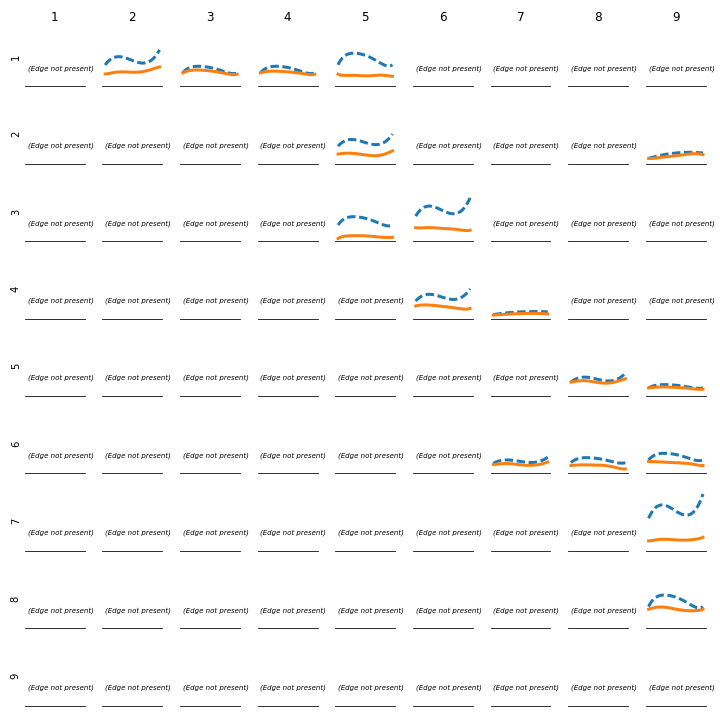
\includegraphics[width=0.8\textwidth]{includes/graphmatrix.png}
\caption{\label{fig:orgparagraph2}
Entry \((i, j)\) is a plot in time of the capacity \(b_{ij}(t)\) (dotted-lines) and the optimal polynomial flow of degree at most \(9\) \(f_{ij}(t)\) (in full lines).}
\end{figure}



In order to know if this can be improved a lot by allowing a higher upper bound on the degree of the polynomial solution, we consider the corresponding time-varying min-cut problem, whose objective value provides an upper bound on the objective value of \ref{eq:orglatexenvironment9}:

\begin{equation*}
\label{eq:orglatexenvironment11}
\tag{MINCUT}
\begin{array}{ll@{}ll}
\underset{(d_{ij}(t))_{ij \in E}, (p_i(t))_{i \in E}}{\text{maximize}} & \int_{-1}^1  \sum_{(i,j) \in E} b_{ij}(t) d_{ij}(t) dt & \\
\text{subject to}& d_{ij}(t) - p_i(t) + p_j(t)  \geq 0 & \forall (i, j) \in E & \; \forall t \in [-1, 1]\\
&p_1(t) - p_n(t) \geq 1 && \; \forall t \in [-1, 1] \\
&p_i(t) \geq 0 & \forall i \in V & \; \forall t \in [-1, 1]\\
& d_{ij}(t)  \geq 0 & \forall (i, j) \in E & \; \forall t \in [-1, 1]
\end{array}
\end{equation*}

We turn this optimization problem into an SDP using the same techniques that we use for \ref{eq:orglatexenvironment9}. Allowing polynomial solutions of degree up to 9, we get an upper bound of \(85.52\) on the optimal value of \ref{eq:orglatexenvironment9}.
\newpage


\subsection{Wireless Coverage problem}
\label{sec:orgheadline22}
In this problem we have two wireless electromagnetic transmitters located at positions \(\bar T_1 = (\bar x_1, \bar y_1)\) and \(\bar T_2 = (\bar x_2, \bar y_2)\). Each transmitter \(i = 1, 2\) is an omnidirectional power source emitting energy \(E_i(t, x, y)\) at time \(t\) in the location \((x, y)\) of space. Electromagnetics laws give the following expression for \(E_i\), \(i=1,2\):

$$E_i(x, y, t)= \frac{c_i(t)}{(x - \bar x_i)^2 + (y - \bar y_i)^2}$$

\noindent where \(c_i(t)\) is the transmission power of the transmitter \(i\) at time \(t\), also equal to the power needed to run the transmitter.

For \(j=1, 2\), we define the regions  \(\mathcal B_j\) by \(k_j\) polynomial inequalities, where \(k_j \in \mathbb N\):
$$\mathcal B_j = \{ (x, y, t) \in \mathbb R^2 \times \mathbb R^2 \times [-1, 1] |\quad  g_{j, 1}(x, y, t) \ge 0, \ldots, g_{j, k_j}(x, y, t) \ge 0\}.$$

Our goal is to make the total energy \(E(x, y, t) = E_1(x, y, t) + E_2(x, y, t)\) at time \(t\) greater than some fixed positive threshold \(C\) for each \((x, y, t) \in \mathcal B_1 \cup \mathcal B_2\) while minimizing the total cost \(\int_{-1}^1 c_1(t) + c_2(t) dt\).

To fix ideas, we take the following numerical example. We fix the required coverage level \(C\) to 1 without loss of generality, and we let the positions of the transmitters to be \(\bar T_1 = (0, 0)\) and \(\bar T_2 = (5, 5)\). The regions \(\mathcal B_1\) and \(\mathcal B_2\) are circles of radius \(1\) and centers \(z_1(t)\) and \(z_2(t)\) moving polynomially in time, i.e.
$$\mathcal B_j = \{(x, y, t), \quad ||\begin{pmatrix}x\\y\end{pmatrix} - z_j(t)|| \le 1\}, j=1,2.$$
\noindent where the centers \(z_1(t), z_2(t)\) are defined as \(z_1(t) \coloneqq  \begin{pmatrix}\frac t3+1\\(\frac t3)^2-1\end{pmatrix}\), \(z_2 \coloneqq \begin{pmatrix}-\frac t3-1\\(\frac t3)^2-1\end{pmatrix}\).

We can formulate the problem as a time-varying optimization problem in the variables \((c_1, c_2)\):


\begin{equation*}
\begin{array}{ll@{}ll}
\underset{(c_1, c_2) \in \mathbb R[t]}{\text{minimize}} && \int_{-1}^1 (c_1(t) + c_2(t)) dt \\
\text{subject to}&&&\\
&c_1(t) &\le \gamma_i & i =1, 2 \quad \forall t \in [-1, 1]\\
&E(x, y, t) &= \sum_{i=1}^2 \frac{c_i(t)}{(x - \bar x_i)^2 + (y - \bar y_i)^2} \ge C & \forall (x, y, t) \in \mathcal B_j
\end{array}
\end{equation*}


Notice that the last inequality can be formulated equivalenty as a polynomial inequality:

$$p(x, y, t) \coloneqq -C \prod_{i=1}^2 [(x - \bar x_i)^2 + (y - \bar y_i)^2] + \sum_{i=1}^2  [(x - \bar x_i)^2 + (y - \bar y_i)^2] c_i(t) \ge 0 \quad \forall (x, y, t)\in \mathcal B_1 \cup \mathcal B_2.$$

We relax the non-negativity constraint to \(p(x, y, t)\) being sum of squares polynomials, i.e:

$$p = \sigma_0^{(j)} + (1-t) \sigma_1^{(j)} + (1+t) \sigma_2 + \mu_1^{(j)} (1 - (x - \bar x_1)^2 - (y - \bar y_1)^2 ) \quad j=1,2$$

\noindent where \(\sigma_0^{(j)}, \sigma_1^{(j)}, \sigma_2^{(j)}, \mu_1^{(j)}, \mu_2^{(j)}\) are sum of squares polynomials in the variables \(x, y\) and \(t\) whose degrees is upper bounded by some integer \(d\).


Written in this form, this is a time-varying SDP that is strictly feasible, so Theorem \ref{orgspecialblock18} implies that polynomial solutions are near optimal.

Table \ref{tbl:wireless} reports the optimal values found for \(d=0, 1, 2, 7\).

A version of this problem where the transmission  power \(c_i\) doesn't depend on \(t\) appeared in \cite{ahmadi2016}, which corresponds to \(d=0\). Below we report the optimal solution  we get for \(d=0, 1, 2, 7\).


\begin{table}[H]
\TABLE{\label{tbl:wireless} Optimal values}
{\begin{tabular}{|l|l|l|l|}\hline
$d$ & $c1(t)$ & $c2(t)$ & $\int_{-1}^1 (c_1(t) + c_2(t)) dt$\\\hline
0 & 31.96 & 21.63 & 107.19\\
1 & $28.97+4.07t$ & $24.23-3.7t$ & 106.38\\
2 & $26.67+6.1t+0.47 t^2$ & $25.78-5.82t+0.44t^2$ & 105.49\\
7 & $26.21+7.49 t+0.43 t^2-3.27 t^3+2.95 t^4-0.15 t^5-0.63 t^6$ & $26.18+7.16t+0.81t^2+3.02 t^3-3.38 t^4+0.44 t^5+0.63 t^6$  & 105.42\\
\hline
\end{tabular}}
{}
\end{table}

\begin{figure}[htp]
\centering
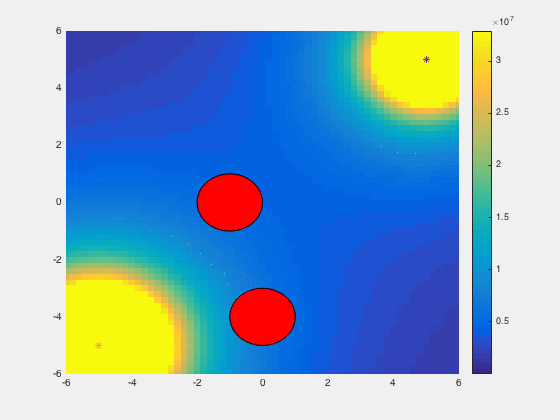
\includegraphics[width=.3\textwidth]{includes/wireless-0.png}\quad
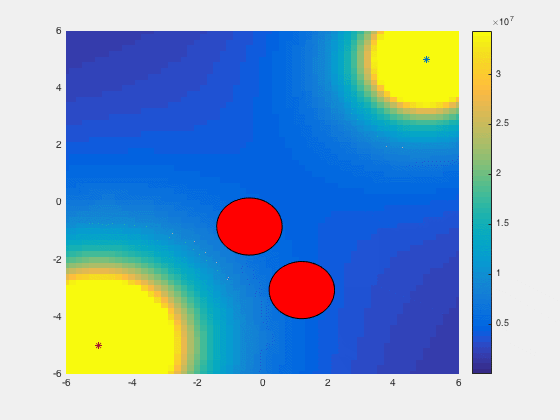
\includegraphics[width=.3\textwidth]{includes/wireless-2.png}
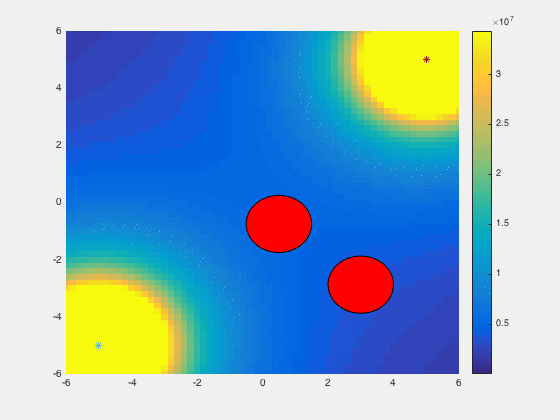
\includegraphics[width=.3\textwidth]{includes/wireless-5.png}

\label{img:wireless}
\caption{An instance of the time-varying wireless coverage problem.}

\end{figure}
\newpage

\section{Conclusion and open questions}
\label{sec:orgheadline24}

This paper presented a natural method to optimize over polynomial solutions to time-varying convex program using the sum of squares framework. We note that even though there exist polynomial algorithms for sum of squares optimization, the best known algorithms scale very poorly as the number of variables the polynomials depend on grow. One notable exception is certifying non-negativity of univariate polynomials, which can be done efficiently using an appropriate basis. We exploit this fact in the case of time-varying linear programs.

The paper also provided sufficient conditions under which polynomial solutions are optimal. It is worth mentioning that the main characterization given here might be asking for too much in certain cases, since it doesn't cover the case of \emph{equality constraints}.


\bibliographystyle{plain}
\bibliography{citations}
\end{document}